\documentclass[12pt, bibliography=totoc, a4paper, abstractoff, numbers=noenddot]{scrreprt}

% define used packages
\usepackage[left=4.0cm, right=2.0cm, top=3cm, bottom=3cm]{geometry}
\usepackage{bibgerm}
\usepackage[utf8]{inputenc}
\usepackage[T1]{fontenc}
\usepackage{graphicx}
\usepackage[ngerman]{babel}
\usepackage{lmodern}
\usepackage{listings}
%% ToDo amsthm packages sind nicht in der Standardlatexvorlage vorhanden
\usepackage{amsthm}
%\usepackage{amssymb}
\newtheorem*{definition}{Definition}
\usepackage[numbers]{natbib}
\usepackage{acronym}
\usepackage{enumitem}

\bibliographystyle{alphadin}
\usepackage{float}

\usepackage{lastpage}

% advanced tables
\usepackage{array}

% header and footer
\usepackage{fancyhdr}

% links
\usepackage{url}

% internal links
\usepackage[colorlinks=true ,linkcolor=black,
			anchorcolor=black ,citecolor=black ,filecolor=black,
			menucolor=black ,urlcolor=black]{hyperref}

% mathematical formulas
\usepackage{amsmath, amssymb}

% fancy Diagrams %
\usepackage{tikz}
\usepackage{epstopdf}

% to include images side by side
\usepackage{subfigure}

% for nice bg on title page
\usepackage{eso-pic}
\newcommand\BackgroundPic{%
\put(0,0){%
\parbox[b][\paperheight]{\paperwidth}{%
\vfill
\centering

\includegraphics[width=\paperwidth,height=\paperheight,%
keepaspectratio]{images/Logo_H-BRS_background.pdf}%
\vfill
}}}

%\usepackage{caption}

% define the programming language
\usepackage{listings}
\lstloadlanguages{Java,sh,bash,Haskell,HTML,PHP,XML}
\lstdefinelanguage{console}{
  morekeywords={},
  otherkeywords={warumgehtdasnicht>,\$}
}
\newcommand{\lstsetconsole}
{ \lstset{%language=sh,
        lineskip=-2pt,
        breaklines=true,
        language=console,
        breaklines=true,
        captionpos=b,
        commentstyle=\textit,
        keywordstyle=\bfseries,
        basicstyle=\ttfamily,
        stringstyle=\ttfamily,
        showstringspaces=false,
        frame=single,
        tabsize=2
  }
}
\lstdefinelanguage{scalaconsole}{
  morekeywords={},
  otherkeywords={scala>,\|}
}
\newcommand{\lstsetrepl}
{ \lstset{%language=sh,
        lineskip=-2pt,
        breaklines=true,
        language=scalaconsole,
        breaklines=true,
        commentstyle=\textit,
        keywordstyle=\bfseries,
        basicstyle=\ttfamily,
        stringstyle=\ttfamily,
        showstringspaces=false,
        frame=single,
        tabsize=2
  }
}
\newcommand{\lstsetjava}{
 \lstset{language=Java,
        breaklines=true,
        commentstyle=\textit,
        keywordstyle=\bfseries,
        basicstyle=\ttfamily,
        stringstyle=\ttfamily,
        showstringspaces=false,
        frame=single,
        captionpos=b,
        tabsize=2,
        literate=
        %linewidth=\textwidth,captionpos=b
        %numbers=left, stepnumber=5, numbersep=10pt
 }
}
\lstdefinelanguage{scala}{
  morekeywords={abstract,case,catch,class,def,%
    do,else,extends,false,final,finally,%
    for,forSome,if,implicit,import,lazy,match,mixin,%
    new,null,object,override,package,%
    private,protected,requires,return,sealed,%
    super,this,throw,trait,true,try,%
    type,val,var,while,with,yield},
  otherkeywords={_,:,=,=>,<-,<\%,<:,>:,\#,@},
  sensitive=true,
  morecomment=[l]{//},
  morecomment=[n]{/*}{*/},
  morestring=[b]",
  morestring=[b]',
  morestring=[b]"""
}
\newcommand{\lstsetscala}{
 \lstset{language=scala,
        breaklines=true,
        commentstyle=\textit,
        keywordstyle=\bfseries,
        basicstyle=\ttfamily,
        stringstyle=\ttfamily,
        showstringspaces=false,
        frame=single,
        tabsize=2
        %%linewidth=\textwidth,captionpos=b
        %numbers=left, stepnumber=5, numbersep=10pt
 }
}
\newcommand{\lstsethtml}{
 \lstset{language=HTML,
        breaklines=true,
        commentstyle=\textit,
        keywordstyle=\bfseries,
        basicstyle=\ttfamily,
        stringstyle=\ttfamily,
        showstringspaces=false,
        frame=single,
        tabsize=2
        %%linewidth=\textwidth,captionpos=b
        %numbers=left, stepnumber=5, numbersep=10pt
 }
}
\newcommand{\lstsetphp}{
 \lstset{language=PHP,
        breaklines=true,
        commentstyle=\textit,
        keywordstyle=\bfseries,
        basicstyle=\ttfamily,
        stringstyle=\ttfamily,
        showstringspaces=false,
        frame=single,
        tabsize=2
        %%linewidth=\textwidth,captionpos=b
        %numbers=left, stepnumber=5, numbersep=10pt
 }
}
\lstnewenvironment{code}
    {\lstset{}%
      \csname lst@SetFirstLabel\endcsname}
    {\csname lst@SaveFirstLabel\endcsname}
\newcommand{\lstsethaskell}{
    \lstset{
      language=Haskell,
      commentstyle=\textit,
      keywordstyle=\bfseries,
      basicstyle=\ttfamily,
      stringstyle=\ttfamily,
      showstringspaces=false,
      frame=single,
      flexiblecolumns=false,
      basewidth={0.5em,0.45em},
      literate={+}{{$+$}}1 {/}{{$/$}}1 {*}{{$*$}}1 {=}{{$=$}}1
               {==}{{$==$}}2 %{!=}{{$\not\equiv$}}2
               {>}{{$>$}}1 {<}{{$<$}}1 {\\}{{$\lambda$}}1
               {\\\\}{{\char`\\\char`\\}}1
               {->}{{$\rightarrow$} }2 {>=}{{$\geq$}}2 {<-}{{$\leftarrow$}}2
               {<=}{{$\leq$}}2 {=>}{{$\Rightarrow$} }2
               {\ .}{{$\circ$}}2 {\ .\ }{{$\circ$}}2 {(.)}{({$\circ$})}2
               {>>}{{>>}}2 {>>=}{{>>=}}2
               {|}{{$\mid$}}1
    }
}
\lstdefinelanguage{JavaScript}{
  keywords={typeof, new, true, false, catch,%
    function, return, null, catch, switch, var,%
    if, in, while, do, else, case, break},
  ndkeywords={class, export, boolean, throw, implements, import, this},
  sensitive=false,
  comment=[l]{//},
  morecomment=[s]{/*}{*/},
  morestring=[b]',
  morestring=[b]"
}
\newcommand{\lstsetjavascript}{
  \lstset{
		language=JavaScript,
		breaklines=true,
		commentstyle=\textit,
		basicstyle=\ttfamily,
		keywordstyle=\bfseries,
		stringstyle=\ttfamily,
		showstringspaces=false,
		frame=single,
		tabsize=2
  }
}
\newcommand{\lstsetxml}{
 \lstset{language=XML,
        breaklines=true,
        commentstyle=\sffamily,
        keywordstyle=\bfseries,
        basicstyle=\sffamily,
        showstringspaces=false,
        stringstyle=\ttfamily,
        frame=single,
        tabsize=2,
        literate=
        %linewidth=\textwidth,captionpos=b
        %numbers=left, stepnumber=5, numbersep=10pt
 }
}
\lstdefinelanguage{CSharp}{
 morekeywords = {abstract,event,new,struct,as,explicit,%
    null,switch,base,extern,object,this,bool,false,%
    operator,throw,break,finally,out,true,byte,fixed,%
    override,try,case,float,params,typeof,catch,for,%
    private,uint,char,foreach,protected,ulong,checked,%
    goto,public,unchecked,class,if,readonly,unsafe,%
    const,implicit,ref,ushort,continue,in,return,using,%
    decimal,int,sbyte,virtual,default,interface,sealed,%
    volatile,delegate,internal,short,void,do,is,sizeof,%
    while,double,lock,stackalloc,else,long,static,%
    enum,namespace,string,partial},
  morecomment = [l]{//},
  morecomment = [l]{///},
  morecomment = [s]{/*}{*/},
  morestring=[b]",
  sensitive = true
}
\newcommand{\lstsetcsharp}{
 \lstset{language=csharp,
        breaklines=true,
        commentstyle=\sffamily,
        basicstyle=\sffamily,
        keywordstyle=\bfseries,
        stringstyle=\ttfamily,
        showstringspaces=false,
        frame=single,
        tabsize=2
        %%linewidth=\textwidth,captionpos=b
        %numbers=left, stepnumber=5, numbersep=10pt
 }
}
\lstdefinelanguage{FSharp}{
  morekeywords={abstract,and,as,assert,base,begin,%
    class,default,delegate,do,done,downcast,downto,%
    elif,else,end,exception,extern,false,finally,for,fun,%
    function,if,in,inherit,inline,interface,internal,lazy,%
    let,match,member,module,mutable,namespace,%
    new,not,null,of,open,or,override,private,public,rec,%
    return,static,struct,then,to,true,try,type,upcast,use,%
    val,void,when,while,with,yield,asr,land,lor,lsl,lsr,lxor,%
    mod,sig,atomic,break,checked,component,const,%
    constraint,constructor,continue,eager,event,external,%
    fixed,functor,global,include,method,mixin,object,%
    parallel,process,protected,pure,sealed,tailcall,trait,virtual,volatile},     
  sensitive=false,
  morecomment=[l][\color{greencomments}]{///},
  morecomment=[l][\color{greencomments}]{//},
  morecomment=[s][\color{greencomments}]{{(*}{*)}},
  morestring=[b]"
}
\newcommand{\lstsetfsharp}{
 \lstset{language=fsharp,
        breaklines=true,
        commentstyle=\sffamily,
        basicstyle=\sffamily,
        keywordstyle=\bfseries,
        stringstyle=\ttfamily,
        showstringspaces=false,
        frame=single,
        tabsize=2
        %%linewidth=\textwidth,captionpos=b
        %numbers=left, stepnumber=5, numbersep=10pt
 }
}

%set default pagestyle
\pagestyle{empty}

\setlength{\parindent}{0pt}
\setlength{\parskip}{12pt}

% #####
% #
% # START config area
% #
% #####

\newcommand{\HEADER}[0]{H-BRS, WS 2018 / 2019}
\newcommand{\PAGENUMBERS}[0]{\pagemark}
\newcommand{\DATE}[0]{12.11.2018}

\newcommand{\AUTHOR}[0]{Rolf Kimmelmann, Jennifer Wittling, Jan Löffelsender}
%\newcommand{\MATNR}[0]{123456}
%\newcommand{\STREET}[0]{Musterstraße 11}
%\newcommand{\ZIP}[0]{12345}
\newcommand{\TOWN}[0]{Sankt Augustin}

\newcommand{\REFERENT}[0]{Prof. Dr. Harm Knolle}
%\newcommand{\KOREFERENT}[0]{Prof. Dr. Max Mustermann}

\newcommand{\TITLE}[0]{PostgresSQL - Rekursion auf Basis generischer Stored Procedures}
%\newcommand{\COURSE}[0]{Master of Science Informatik}
\newcommand{\TYPE}[0]{Projektarbeit}
%\newcommand{\COMPLETION}[0]{Bachelor / Master of Science}

% #####
% #
% # END config area
% #
% #####

% Hurenkinder und Schusterjungenregelung
\clubpenalty=100000
\widowpenalty=100000
\displaywidowpenalty=100000

% starting the document
\begin{document}

% set pagenumbering to roman(I II III IV)
\pagenumbering{Roman}
% input the title
% #####
% #
% # This is the titlelayout from Prof. Dr. Harm Knolle 
% # (Hochschule Bonn-Rhein-Sieg)
% #  
% #####

% #####
% #
% # Default layout
% #
% #####

\AddToShipoutPicture*{\BackgroundPic}

\begin{titlepage}
  \begin{center}
  	
\includegraphics[scale=1]{./images/Logo_H-BRS.jpg}
  \end{center}
  \vspace{40pt}
  \sffamily
  \begin{tabular}{|l>{\raggedright\hspace{0pt}\arraybackslash}p{15cm}}
    & \\
    & \large\textbf{\TYPE}\\[\baselineskip]
    & \huge\textbf{\TITLE}\\[\baselineskip]
%    & \textbf{Falls erforderlich: Zur Erlangung des akademischen Grades eines}\\
%    & \COMPLETION\\
%    & - \COURSE\ -\\
    & \\
  \end{tabular}
  \vfill
  \begin{tabular}{ll@{}}
    & Fachbereich Informatik\\[\baselineskip]
    &   Referent: \REFERENT\\[\baselineskip]
%    &   Falls erforderlich: Korreferent: \KOREFERENT\\[\baselineskip]
    & \\[\baselineskip]
    & eingereicht von:\\[\baselineskip]
    & \AUTHOR\\[\baselineskip]
%    & Matr.-Nr. \MATNR\\[\baselineskip]
%    & \STREET\\[\baselineskip]
%    & \ZIP \ \TOWN\\[\baselineskip]
    & \\[\baselineskip]
    & Sankt Augustin, den \DATE\\[\baselineskip]
  \end{tabular}
\end{titlepage}

\nocite{*} %TODO: Show full bibliography remove for final version.  

% Inhaltsverzeichnis

	%\setcounter{tocdepth}{1}
	%für die Anzeige von Unterkapiteln im Inhaltsverzeichnis
\setcounter{tocdepth}{2}
\newpage


%Inhalt
\begin{abstract}
\section*{Exposé}\markboth{Exposé}{}
  \addcontentsline{toc}{chapter}{Exposé}Lorem ipsum dolor sit amet, consetetur sadipscing elitr, sed diam nonumy eirmod tempor invidunt ut labore et dolore magna aliquyam erat, sed diam voluptua. At vero eos et accusam et justo duo dolores et ea rebum. Stet clita kasd gubergren, no sea takimata sanctus est Lorem ipsum dolor sit amet. Lorem ipsum dolor sit amet, consetetur sadipscing elitr, sed diam nonumy eirmod tempor invidunt ut labore et dolore magna aliquyam erat, sed diam voluptua. At vero eos et accusam et justo duo dolores et ea rebum. Stet clita kasd gubergren, no sea takimata sanctus est Lorem ipsum dolor sit amet. Lorem ipsum dolor sit amet, consetetur sadipscing elitr, sed diam nonumy eirmod tempor invidunt ut labore et dolore magna aliquyam erat, sed diam voluptua. At vero eos et accusam et justo duo dolores et ea rebum. Stet clita kasd gubergren, no sea takimata sanctus est Lorem ipsum dolor sit amet.

Duis autem vel eum iriure dolor in hendrerit in vulputate velit esse molestie consequat, vel illum dolore eu feugiat nulla facilisis at vero eros et accumsan et iusto odio dignissim qui blandit praesent luptatum zzril delenit augue duis dolore te feugait nulla facilisi. Lorem ipsum dolor sit amet, consectetuer adipiscing elit, sed diam nonummy nibh euismod tincidunt ut laoreet dolore magna aliquam erat volutpat. 

Ut wisi enim ad minim veniam, quis nostrud exerci tation ullamcorper suscipit lobortis nisl ut aliquip ex ea commodo consequat. Duis autem vel eum iriure dolor in hendrerit in vulputate velit esse molestie consequat, vel illum dolore eu feugiat nulla facilisis at vero eros et accumsan et iusto odio dignissim qui blandit praesent luptatum zzril delenit augue duis dolore te feugait nulla facilisi. 

Nam liber tempor cum soluta nobis eleifend option congue nihil imperdiet doming id quod mazim placerat facer possim assum. Lorem ipsum dolor sit amet, consectetuer adipiscing elit, sed diam nonummy nibh euismod tincidunt ut laoreet dolore magna aliquam erat volutpat. Ut wisi enim ad minim veniam, quis nostrud exerci tation ullamcorper suscipit lobortis nisl ut aliquip ex ea commodo consequat. 

Duis autem vel eum iriure dolor in hendrerit in vulputate velit esse molestie consequat, vel illum dolore eu feugiat nulla facilisis. 
\end{abstract}

% set pagenumbering to arabic(1 2 3 4)
\pagenumbering{arabic}
\tableofcontents

%% Document
\chapter*{Beispielgliederung}
%    \section*{beispielgliederung}\markboth{beispielgliederung}{}
%    \addcontentsline{toc}{chapter}{beispielgliederung}
    \begin{enumerate}
        \item Graph-Datenbanken - Grundlegende technologische Aspekte
        \begin{enumerate}[label*=\arabic*.]
            \item Einführung
            \item Modell (Graph, Property Graphen, Hypergraphen)
        \end{enumerate}
        \item Graph-Datenbanken und -Frameworks - PostgresSQL
        \begin{enumerate}[label*=\arabic*.]
            \item Allgemein
            \item Architektur
            \item Datenmodell
            \item Indexe
            \item Anfragemethoden
            \item Konsistenz
        \end{enumerate}
        \item Graph-Datenbanken im praktischen Einsatz: OLTP
            \begin{enumerate}[label*=\arabic*.]
                \item Ausgewählte Use Cases
                \item Weitere Zugriffstechniken
                \item Vergleich mit relationalen Datenbanksystemen
                \item Beurteilung
            \end{enumerate}
        \item Graph-Datenbanken im praktischen Einsatz: OLAP
        \begin{enumerate}[label*=\arabic*.]
            \item Benchmark
            \item Datenbankzugriffe
            \item Zugriffsart Aggregation
            \item Zugriffsart Traversierung
            \item Interpretation der Ergebnisse
        \end{enumerate}
    \end{enumerate}

%\end{beispielgliederung}
\chapter{Graph-Datenbanken - Grundlegende technologische Aspekte}
\section{Einführung}
\section{Modell}
\subsection{Graph}
Ein Graph G besteht aus einer nichtleeren Menge an Knoten V und Kanten E (G = (V,E)).
Die Kanten stellen die Beziehung zwischen den einzelnen Knoten her.
In einem klassischen Graphen kann eine Kante immer nur jeweils zwei Knoten miteinander verbinden.
Graphen können gerichtet oder ungerichtet sein. Gerichtete Graphen zeichnen sich dardurch aus, dass die Kanten eine zugewiesen Richtung besitzen.
Um die Beziehung zwischen zwei Knoten genauer zu definieren lassen sich die Kanten gewichten.
In diesem Fall werden den Kannten in der Regel nummerische Werte zugeordnet und man bezeichnet diese Graphen als Gewichtete Graphen.
Werden Kanten und Knoten eines Graphs vertauscht entsteht der Kantengraph bzw. Line-Graph des jeweiligen Graphen L(G).
Zwei Graphen können isomorph sein.
\\Verschiedene Graphen:
\begin{itemize}
	\item Planare Graphen
	\subitem lassen sich in der Ebene ohne Überschneidung der Kanten zeichnen\cite{Theobald2016}
	\item Reguläre Graphen
	\subitem alle Knoten haben den selben Knotengrad
	\item Partite Graphen
	\subitem die Knoten können in verschiedene Partitionen unterteilt werden
	\item Multimodale Graphen
\end{itemize}

%\\Ein Graph ist mathematisch folgendermaßen definiert: \\
%\begin{definition}
%	Ein $\text{Graph(graph)}G=(V,E,\gamma)$ ist ein Tripel bestehend aus:
%	\begin{itemize}
%		\item $V$, einer nicht leeren Menge von Knoten(vertices)
%		\item $E$, einer Menge von Kanten (edges) und
%		\item $\gamma$ , einer Inzidenzabbildung (incidence relation), mit\\
%		$\gamma : E \longrightarrow \{X | X \subseteq V, 1 \leq |X| \leq 2\}$
%	\end{itemize}
%	Zwei Knoten $a,b \in V$ heißen adjazent(adjacent) genau dann wenn
%	$\exists e \in E: \gamma(e)=\{a,b\}$. \\
%	Ein Knoten $a \in V$ und eine Kante $e \in E$ heißen inzident (incident)
%	genau dann wenn $a \in \gamma(e)$. \footnote{Vgl. \cite[Seite 21]{pbeck01}}
%\end{definition}
\subsection{Property Graphen}
Property Graphen zeichnen sich durch ihre den Kanten und Knoten zugewiesenen Eigenschaften auf.
\subsection{Hypegraphen}
Hypergraphen haben die Eigenschaft, dass Kanten im Gegensatz zu klassischen Graphen mehr als zwei Knoten miteinander verbinden können.
\\Mathematisch ist ein Hypergraph ist folgendermaßen definiert:
\begin{definition}
	Let $X=\{v_{1}, v_{2},...,v_{n}\}$ be a finite set,
	and let $E=\{e_{1},e_{2},...,e_{m}\}$ be a family of subsets of $X$ such that
	\[e_{i} \neq \varnothing (i=1,2,...,m) \\
	\cup_{i=1}^{m}e_{i}=X.
	\]
	The pair $H=(X,E)$ is called a hypergraph with vertex set $X$
	and hyperedge set $E$. The elements $v_{1}, v_{2},...,v_{n}$ of $X$ are vertices
	of hypergraph $H$, and the sets $e_{1}, e_{2},...,e_{m}$ are hyperedges of hypergraph $H$.\footnote{Vgl. \cite[Seite 2]{zhang2018hypergraph}}
\end{definition}

Das folgende Bild zeigt einen Hypergraphen:

\begin{center}
	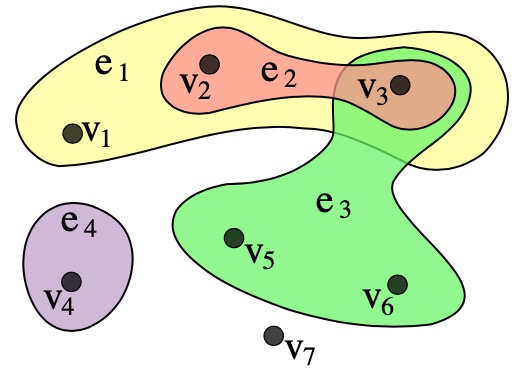
\includegraphics[scale = 0.5]{./images/Hypergraph.jpg}
\end{center}
Im Vergleich zum normale Graphen können die Kanten eines Hypergraphen eine beliebige Kardinalität haben (siehe Definition Definition Graph Kapitel 1.2.1) . Beim normalen Graphen können die Kanten nur die Kardinalität $1 \leq |X| \leq 2$
haben. Die Hyperedges in einem Hypergraphen sind somit eine beliebige Menge von Knoten. In einem normale Graphen sind die Kanten, eine in einem Intervall festgelegte Menge von Knoten:
    \[X = \{v_{1}, v_{2}, v_{3}, v_{4}, v_{5}, v_{6}, v_{7}\} \text{ Knoten}\]
    \[E=\{e_{1}, e_{2}, e_{3}, e_{4}\} \text{ Kanten}\]
    \[E=\{e_{1}, e_{2}, e_{3}, e_{4}\} = \{\{v_{1}, v_{2}, v_{3}\}, \{v_{2}, v_{3}\}, \{v_{3}, v_{5}, v_{6}\}, \{v_{4}\}\} \]
\chapter{Graph-Datenbanken und -Frameworks - Ausgewählte Systeme }
\section{PostgreSQL}
\subsection{Allgemein}
    \begin{itemize}
        \item Kategorie / Modell
            \subitem PostgreSQL ist ein Relationales Datenbank System \cite{postgresqldoc}
        \item Version
            \subitem Aktuelle Major Version: 11
        \item Historie
            \subitem PostgreSQL ist aus dem POSTGRES projekt der University of California at Berkeley entstanden, welches unter der Leitung von  Professor Michael Stonebraker im Jahre 1986 began.
            SQL Interpreter seit 1994, das System hieß zu diesem Zeitpunkt Postgres95. 1996 wurde es in PostgrSQL umbenannt.\cite{postgresqldoc}
        \item Hersteller
        \item Lizenz
            \subitem Open-Source
    \end{itemize}
\subsection{Architektur}
    \begin{itemize}
        \item Programmiersprache des Systems
        \item Systemkomponenten, Systemarchitektur
        \subitem client / server Architektur \cite{postgresqldoc}
        \item Betriebsart
            \subitem Cluster - Menge an Datenbanken, die von PostSQL-Server verwaltet werden \cite{froehlich01}
        \item Protokoll der Schnittstelle
        \subitem TCP/IP
        \item API
    \end{itemize}
    Die Architektur von PostgresSQL ist in folgendem Bild gegeben:
    \begin{center}
        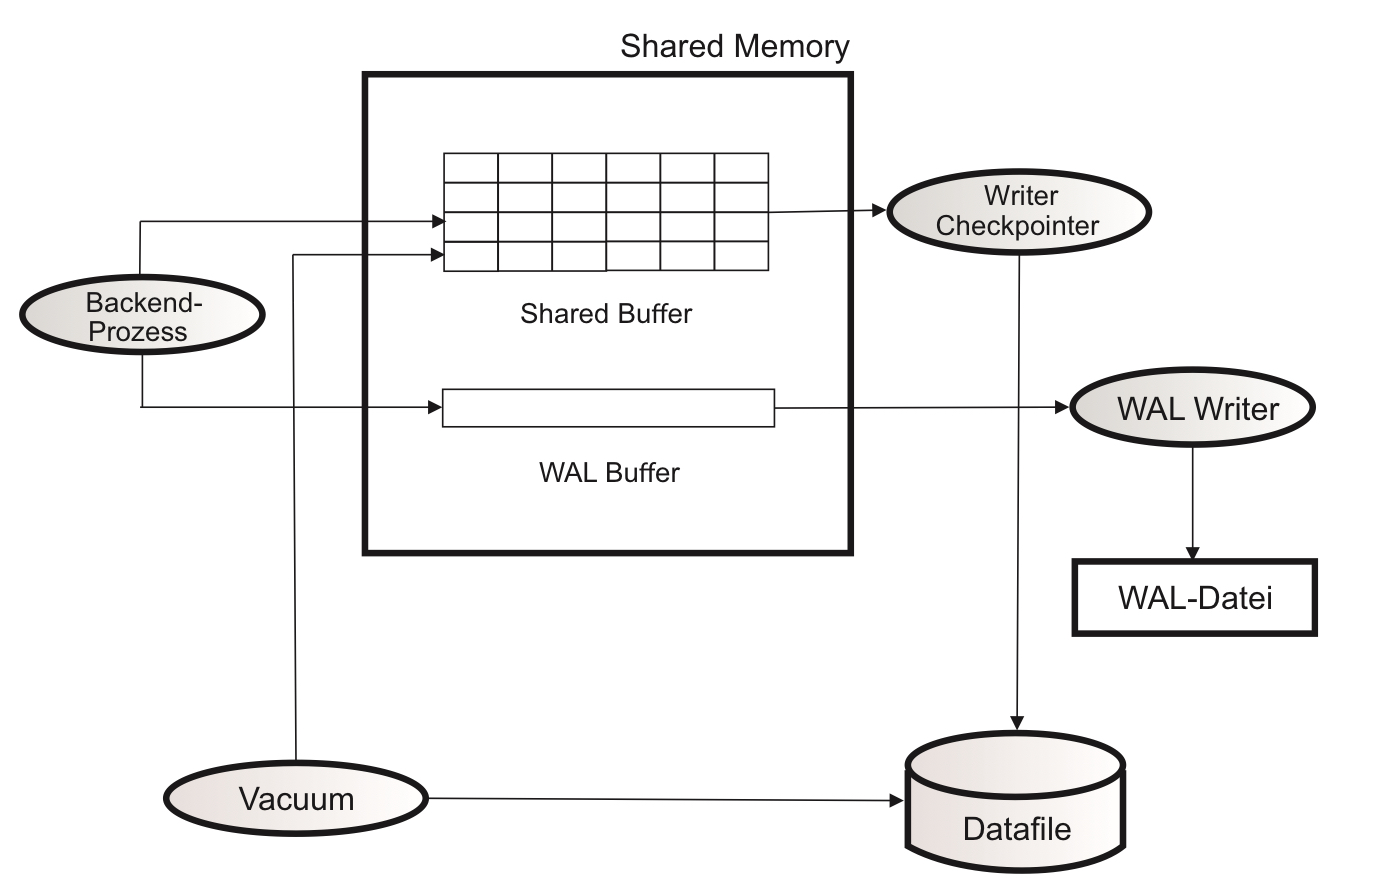
\includegraphics[width = \linewidth]{./images/PostgresSQLArchitektur.jpg}
    \end{center}
    Diese Architektur ergibt sich aus der Gegebenheit, dass alle Daten normalerweise nicht in den Shared Buffer passen. Ein Teil der Datenbank befindet sich im Datafile, aus der bei Bedarf gelesen werden kann, der andere Teil im Shared Buffer.
    Die Hauptaufgabe des Shared Buffer ist es, Input Output Operationen (I/O Operationen) auf das Datafile zu minimieren und möglichst viele Operationen im Speicher durchzuführen. Die Motivation möglichst viele Operation im Speicher durchzuführen
    besteht darin, dass Operationen im Speicher schneller ausgeführt werden. Werden Operationen im Speicher ausgeführt, so werden I/O Operationen auf das Datafile reduziert. Der Writer Prozess ist für die Synchronisation
    des Zustands des Shared Buffers und der Tablespaces verwantwortlich. Dieser Prozess schreibt Datenblöcke aus dem Shared Buffer auf die Tablespaces innerhalb des Datafile. Der Writer Checkpoint ist dafür verantwortlich,
    dass alle geänderten Datenblöcke innerhalb des Shared Buffer in das Datafile geschrieben werden. \footnote{Vgl. \cite[Seite 26]{froehlich01}} \\
    Eine PostgreSQL-Instanz wird als Server Prozess mit eigenem Datenverzeichnis und einer eigenen Konfigurationsdatei sowie einem eigenen Transaktionslog.
\subsection{Datenmodell}
    \begin{itemize}
        \item Standardsprache: SQL
        \item Objektbegriff, Konzepte: Relationale Datenbank - Abbildung in Tabellen
        \item Datentypen:
        \subitem Sehr viele unterstützte Datentypen, es lassen sich aber auch eigene Datentypen mittesl des CREATE TYPE befehls erstellen.\cite{postgres8}
    \end{itemize}
    Daten werden in Form von Tabellen abgelegt. Im Filesystem legt PostgreSQL Dateien im sogenannten \$PGDATA-Verzeichnis ab, dieses wird beim Start von PostgreSQL festgelegt. Alle Date werden im Verzeichnis Base unterhalb von \$PGDATA abgelegt. Einzelne Tabellen oder Indices können in Tablespaces ausgelagert werden. Für einen Tablespace wird ein neuer Unterordner im \$PGDATA-Verzeichnis angelegt. Es ist auch möglich einzelne Spalten einer Tabelle in einen anderen Tablespace zu verschieben.
\subsection{Konsistenz}
PostgreSQL ist eine Objektrelationale Datenbank. Weiterentwicklungen wird von der PostgreSQL Global Development Group durchgeführt. PostgreSQL steht unter der PostgreSQL-Lizenz, welche sehr stark der GNU-Lizenz ähnelt. Auf Basis von PostgreSQL gibt es mehrere, zum Teil auch kommerzielle, Forks wie zum Beispiel Amazon Redshift oder EnterpriseDB.
PostgreSQL schreibt einen Transaktionslog (Write-Ahead Log, WAL).
Dieser wird als WAL-Buffer im Arbeitsspeicher und als WAL-Dateien auf der Festplatte geführt.
Bei jedem Commit einer Transaktion wird zunächst das WAL aktualisiert bevor die Bestätigung an den Client gesendet wird.
Der walwriter-Prozess schreibt periodisch die WAL-Buffer auf die Festplatte.
\section{Indexe}
\section{Anfragemethoden}
\section{Konsistenz}


\chapter{Graph-Datenbanken im praktischen Einsatz: OLTP}
\section{PostgresSQL: OLTP}
\section{Ausgewählte Use Cases}
\section{Beurteilung}
\chapter{Graph-Datenbanken im praktischen Einsatz: OLAP}
\section{PostgreSQL: OLAP}
\subsection{Benchmark}
Mit der Standardinstallation von PostgreSQL wird auch pgbench mitinstalliert. Bei pgbench handelt es sich um ein einfaches Tool zur Durchführung von Benchmark-Tests. Bei einem Benchmark-Test wird eine Menge von SQL-Statements beliebig oft wiederholt, dabei können auch mehrere parallele Sessions geöffnet werden. Beim durchführen des Tests berechnet pgbench die Anzahl der Transaktionen pro Sekunde.
\subsubsection{Verwendung von pgbench}
pgbench wird über die Kommandozeile gestartet. Dabei können eine Reihe von Parametern übergeben werden, mit denen das Verhalten von pgbench gesteuert werden kann.
\begin{itemize}
	\item -c clients  \\
	Über das Flag -c wird die Anzahl der Clients bzw. die Anzahl der gleichzeitigen Datenbankverbindungen festgelegt. Wenn hier nichts angegeben ist wird nur ein Client verewendet.
	\item -t transactions \\
	Über das Flag -t wird festgelegt wieviele Transaktionen jeder Client durchführt. Die Anzahl aller Transaktionen ergibt sich durch das Produkt von Clients und Transactions.
\end{itemize}
\subsection{Standard SQL}
\subsection{Stored Procedures}
\subsection{PL/SQL-Recursion}
\subsection{Datenbankzugriffe}
\subsection{Zugriffsart Aggregation}
\subsection{Zugriffsart Traversierung}
\subsection{Interpretation der Ergebnisse}
%\chapter*{Graph}
Ein Graph ist mathematisch folgendermaßen definiert: \\
\begin{definition}
    Ein $\text{Graph(graph)}G=(V,E,\gamma)$ ist ein Tripel bestehend aus:
    \begin{itemize}
        \item $V$, einer nicht leeren Menge von Knoten(vertices)
        \item $E$, einer Menge von Kanten (edges) und
        \item $\gamma$ , einer Inzidenzabbildung (incidence relation), mit\\
        $\gamma : E \longrightarrow \{X | X \subseteq V, 1 \leq |X| \leq 2\}$
    \end{itemize}
    Zwei Knoten $a,b \in V$ heißen adjazent(adjacent) genau dann wenn
    $\exists e \in E: \gamma(e)=\{a,b\}$. \\
    Ein Knoten $a \in V$ und eine Kante $e \in E$ heißen inzident (incident)
    genau dann wenn $a \in \gamma(e)$. \footnote{Vgl. \cite[Seite 21]{pbeck01}}
\end{definition}

%\chapter*{Hypergraph}
Ein Hypergraph ist folgendermaßen definiert:
\begin{definition}
Let $X=\{x_{1}, x_{2},...,x_{n}\}$ be a finite set,
and let $E=\{e_{1},e_{2},...,e_{m}\}$ be a family of subsets of $X$ such that
    \[e_{i} \neq \varnothing (i=1,2,...,m) \\
    \cup_{i=1}^{m}e_{i}=X.
    \]
The pair $H=(X,E)$ is called a hypergraph with vertex set $X$
and hyperedge set $E$. The elements $x_{1}, x_{2},...,x_{n}$ of $X$ are vertices
    of hypergraph $H$, and the sets $e_{1}, e_{2},...,e_{m}$ are hyperedges of hypergraph $H$.\footnote{Vgl. \cite[Seite 2]{zhang2018hypergraph}}
\end{definition}


%\end{document}
% load the preamble
%% \renewcommand\abstractname{Danksagung}
\begin{abstract}
\section*{Vorwort}\markboth{Vorwort}{}
  \addcontentsline{toc}{chapter}{Vorwort}
\enlargethispage*{\baselineskip}
%\begin{center}
\begin{figure}[H]
  \begin{table}[H]
  \centering
    \begin{tabular}{|c|l|r|}
      \hline
      Kapitel & Verantwortlicher\\
      \hline
      \hline
      1 & Jennifer Wittling\\
      \hline
      2 & Jan Löffelsender\\
      \hline
      3 & Jan Löffelsender\\
      \hline
      4 & Rolf Kimmelmann\\
      \hline
      %5 & sed diam voluptua & 1005 \\
      %\hline
      %6 & clita kasd gubergren & 1006 \\
      %\hline
    \end{tabular}
    \caption{Aufgabenverteilung}
%    \label{table1}
  \end{table}
\end{figure}
%\end{center}
  Die packages
  \begin{itemize}
    \item amsthm,
    \item lstautogobble,
    \item multirow
  \end{itemize}
  wurden zusaätzlich zur Standardvorlage verwendet.

\end{abstract}

%
%% loads the fancy pagestyle for register part
%% set the pagestyle to fancy
\pagestyle{fancy}

\fancyhf{}% clear all fields
  % define the header
  \fancyhead[L]{\leftmark}% left header
  \fancyhead[R]{\HEADER}% right header
  \renewcommand{\headrulewidth}{0.4pt}% top line

  % define the footer
  \fancyfoot[L]{\AUTHOR}% left footer
  \fancyfoot[R]{\pagemark}% right footer
  \renewcommand{\footrulewidth}{0.6pt}% bottom line

  % redefine the chaptermark to have '1. Chaptername' and not 'CHAPTER 1.
  % CHAPTERNAME'
  \renewcommand{\chaptermark}[1]{\markboth{\thechapter.\ #1}{}}

% override the plain style
\fancypagestyle{plain}{%
\fancyhf{}% clear all fields
  % define the header
  \renewcommand{\headrulewidth}{0.0pt}% top line

  % define the footer
  \fancyfoot[L]{\AUTHOR}% left footer
  \fancyfoot[R]{\pagemark}% right footer
  \renewcommand{\footrulewidth}{0.6pt}% bottom line
}

%
%% create the registers
%\tableofcontents\newpage
%

%\pagenumbering{arabic}
%% loads the fancy pagestyle for main part
%% set the pagestyle to fancy
\pagestyle{fancy}

\fancyhf{}% clear all fields
  % define the header
  \fancyhead[L]{\leftmark}% left header
  \fancyhead[R]{\HEADER}% right header
  \renewcommand{\headrulewidth}{0.4pt}% top line

  % define the footer
  \fancyfoot[L]{\AUTHOR}% left footer
  \fancyfoot[R]{\PAGENUMBERS}% right footer
  \renewcommand{\footrulewidth}{0.6pt}% bottom line

  % redefine the chaptermark to have '1. Chaptername' and not 'CHAPTER 1.
  % CHAPTERNAME'
  \renewcommand{\chaptermark}[1]{\markboth{\thechapter.\ #1}{}}

% override the plain style
\fancypagestyle{plain}{%
\fancyhf{}% clear all fields
  % define the header
  \renewcommand{\headrulewidth}{0pt}% top line

  % define the footer
  \fancyfoot[L]{\AUTHOR}% left footer
  \fancyfoot[R]{\PAGENUMBERS}% right footer
  \renewcommand{\footrulewidth}{0.6pt}% bottom line
}

%
%% #####
%% # load the chapter from the files
%% #
%% # TODO: create new chapter
%% #####
%\chapter{Erstes Kapitel}
Das ist zunächst ein normaler Text ... Lorem ipsum dolor sit amet, consetetur sadipscing elitr, sed diam nonumy eirmod tempor invidunt ut labore et dolore magna aliquyam erat, sed diam voluptua. At vero eos et accusam et justo duo dolores et ea rebum. Stet clita kasd gubergren, no sea takimata sanctus est Lorem ipsum dolor sit amet. Lorem ipsum dolor sit amet, consetetur sadipscing elitr, sed diam nonumy eirmod tempor invidunt ut labore et dolore magna aliquyam erat, sed diam voluptua. At vero eos et accusam et justo duo dolores et ea rebum. Stet clita kasd gubergren, no sea takimata sanctus est Lorem ipsum dolor sit amet. Lorem ipsum dolor sit amet, consetetur sadipscing elitr, sed diam nonumy eirmod tempor invidunt ut labore et dolore magna aliquyam erat, sed diam voluptua. At vero eos et accusam et justo duo dolores et ea rebum. Stet clita kasd gubergren, no sea takimata sanctus est Lorem ipsum dolor sit amet. 

Duis autem vel eum iriure dolor in hendrerit in vulputate velit esse molestie consequat, vel illum dolore eu feugiat nulla facilisis at vero eros et accumsan et iusto odio dignissim qui blandit praesent luptatum zzril delenit augue duis dolore te feugait nulla facilisi. Lorem ipsum dolor sit amet, consectetuer adipiscing elit, sed diam nonummy nibh euismod tincidunt ut laoreet dolore magna aliquam erat volutpat. 

Lorem ipsum dolor sit amet, consetetur sadipscing elitr, sed diam nonumy eirmod tempor invidunt ut labore et dolore magna aliquyam erat, sed diam voluptua. At vero eos et accusam et justo duo dolores et ea rebum. Stet clita kasd gubergren, no sea takimata sanctus est Lorem ipsum dolor sit amet. 
\begin{center}
Der folgende Bereich (Umgebung) \\ 
wird jetzt zentriert (center von begin bis end)
\Large

und zugleich groß (Large)
\tiny

und jetzt zugleich klein (tiny)
\end{center}
Es wird lediglich das folgende Wort
\textsl{kursiv} (textsl, slanted) hervorgehoben. 

Das folgende Word wird \textbf{fett} (textbf, boldface) und jetzt \textsl{\textbf{fett und kursiv}} zugleich dargestellt.

Ein Textbereich kann auch ab jetzt \itshape (z.B. itshape, kursiv) hervorgehoben werden ... solange bis eine andere Hervorhebung wie z.B. das \normalfont Standardformat (normalfont) wieder festgelegt wird. 

Sonderzeichen müssen gekennzeichnet bzw. maskiert werden:

\verb=\=: ganz kompliziert mit \bfseries \verb=\=verb=\verb=\== \normalfont

\verb=~=: ebenfalls kompliziert mit \bfseries \verb=\=verb=\verb=~== \normalfont

Viele Sonderzeichen benötigen jedoch nur ein vorangestelltes \verb=\=:

\%: \bfseries \verb=\=\% \normalfont

\{: \bfseries \verb=\=\{ \normalfont

\_: \bfseries \verb=\=\- \normalfont

Die Befehle für deutsche Anführungszeichen sind Teil des Pakets german, bzw. ngerman. Das untere Anführungszeichen erhält man durch "'`, das obere durch "''.

Die deutschen Umlaute werden durch das Einbinden entsprechender Zusatzmodule (Pachages) für die deutschen Schriftzeichen ermöglicht und können "`einfach so"' benutzt werden: äöüÄÖÜß.

Einen einfachen Umbruch (jetzt)\\ in einem Absatz erreicht man mit \verb=\=\verb=\=. 

Jetzt kommt eine Fußnote.\footnote{http://www.h-brs.de}

\section{Listings}
Jetzt kommen einige Listings, die exakt dort im Text erscheinen, wo sie definiert werden. Das Problem hierbei ist, dass die Listings Opfer des Seitenumbruchs werden können. Abhilfe schafft hier die Option "`float, floatplacement=H"', wodurch das Listing an den Anfang der nächsten Seite gesetzt wird. Bei Tabellen und Abbildungen wird eine andere dynamische Positionierung genutzt (siehe Abbildung \ref{figure01} und Tabelle \ref{table01} im zweiten Kapitel ).

\lstsethaskell
\begin{lstlisting}[float, floatplacement=H, label=listinghaskell, captionpos=b, caption=Beispiel Haskell]
module Main where

-- this is a comment
f :: Show a => a -> Int -> String
f x i = show x ++ show i

main :: IO ()
main = do
  putStrLn "Hello World"
  putStrLn $ f 1.2 3
  print $ sum [1..10]
\end{lstlisting}

Lorem ipsum dolor sit amet, consetetur sadipscing elitr, sed diam nonumy eirmod tempor invidunt ut labore et dolore magna aliquyam erat, sed diam voluptua. At vero eos et accusam et justo duo dolores et ea rebum. Stet clita kasd gubergren, no sea takimata sanctus est Lorem ipsum dolor sit amet.
 
\lstsetjava
\begin{lstlisting}[float, floatplacement=H, label=listingjava,caption=Beispiel Java]
// Comment
class Main {
  public static void main(String[] args) {
    System.out.println("Hello World");
  }
}
\end{lstlisting}

Lorem ipsum dolor sit amet, consetetur sadipscing elitr, sed diam nonumy eirmod tempor invidunt ut labore et dolore magna aliquyam erat, sed diam voluptua. 

\lstsetscala
\begin{lstlisting}[label=listingscala,caption=Beispiel Scala]
// Comment
class Main extends App {
  println("Hello World")
}
\end{lstlisting}

\section{Formeln}

Komplette Referenz zu AMSMath siehe \\
\url{ftp://ftp.ams.org/ams/doc/amsmath/short-math-guide.pdf}

\begin{align}
 \int_{a}^{b} x\,dx
 & = \left.\frac{1}{2} x^2\right\vert_{a}^{b}\\
 & = \frac{1}{2} b^2 - \frac{1}{2} a^2 \\
 \intertext{mit $a=1$ und $b=3$ folgt:}
 \notag
 & = \frac{1}{2} \left(3^2 - 1^2\right)\\
 & = 5
\end{align}

\section{Dritter Abschnitt}
Lorem ipsum dolor sit amet, consetetur sadipscing elitr, sed diam nonumy eirmod tempor invidunt ut labore et dolore magna aliquyam erat, sed diam voluptua. At vero eos et accusam et justo duo dolores et ea rebum. Stet clita kasd gubergren, no sea takimata sanctus est Lorem ipsum dolor sit amet. Lorem ipsum dolor sit amet, consetetur sadipscing elitr, sed diam nonumy eirmod tempor invidunt ut labore et dolore magna aliquyam erat, sed diam voluptua. At vero eos et accusam et justo duo dolores et ea rebum. Stet clita kasd gubergren, no sea takimata sanctus est Lorem ipsum dolor sit amet. Lorem ipsum dolor sit amet, consetetur sadipscing elitr, sed diam nonumy eirmod tempor invidunt ut labore et dolore magna aliquyam erat, sed diam voluptua. At vero eos et accusam et justo duo dolores et ea rebum. Stet clita kasd gubergren, no sea takimata sanctus est Lorem ipsum dolor sit amet. 

Jetzt kommt eine Referenz \cite[Seite 300]{kudrass01}

\section{Vierter Abschnitt}
Lorem ipsum dolor sit amet, consetetur sadipscing elitr, sed diam nonumy eirmod tempor invidunt ut labore et dolore magna aliquyam erat, sed diam voluptua. At vero eos et accusam et justo duo dolores et ea rebum. Stet clita kasd gubergren, no sea takimata sanctus est Lorem ipsum dolor sit amet. Lorem ipsum dolor sit amet, consetetur sadipscing elitr, sed diam nonumy eirmod tempor invidunt ut labore et dolore magna aliquyam erat, sed diam voluptua. At vero eos et accusam et justo duo dolores et ea rebum. Stet clita kasd gubergren, no sea takimata sanctus est Lorem ipsum dolor sit amet. Lorem ipsum dolor sit amet, consetetur sadipscing elitr, sed diam nonumy eirmod tempor invidunt ut labore et dolore magna aliquyam erat, sed diam voluptua. At vero eos et accusam et justo duo dolores et ea rebum. Stet clita kasd gubergren, no sea takimata sanctus est Lorem ipsum dolor sit amet. 

\section{Noch ein Abschnitt}
Lorem ipsum dolor sit amet, consetetur sadipscing elitr, sed diam nonumy eirmod tempor invidunt ut labore et dolore magna aliquyam erat, sed diam voluptua. At vero eos et accusam et justo duo dolores et ea rebum. Stet clita kasd gubergren, no sea takimata sanctus est Lorem ipsum dolor sit amet. Lorem ipsum dolor sit amet, consetetur sadipscing elitr, sed diam nonumy eirmod tempor invidunt ut labore et dolore magna aliquyam erat, sed diam voluptua. At vero eos et accusam et justo duo dolores et ea rebum. Stet clita kasd gubergren, no sea takimata sanctus est Lorem ipsum dolor sit amet. Lorem ipsum dolor sit amet, consetetur sadipscing elitr, sed diam nonumy eirmod tempor invidunt ut labore et dolore magna aliquyam erat, sed diam voluptua. At vero eos et accusam et justo duo dolores et ea rebum. Stet clita kasd gubergren, no sea takimata sanctus est Lorem ipsum dolor sit amet. 

Und noch eine Fußnote, jetzt mit Referenz: \footnote{Vgl. \cite{redmont01}}

\section{Ein Abschnitt zweiten Grades}
Lorem ipsum dolor sit amet, consetetur sadipscing elitr, sed diam nonumy eirmod tempor invidunt ut labore et dolore magna aliquyam erat, sed diam voluptua. At vero eos et accusam et justo duo dolores et ea rebum. Stet clita kasd gubergren, no sea takimata sanctus est Lorem ipsum dolor sit amet. Lorem ipsum dolor sit amet, consetetur sadipscing elitr, sed diam nonumy eirmod tempor invidunt ut labore et dolore magna aliquyam erat, sed diam voluptua. At vero eos et accusam et justo duo dolores et ea rebum. Stet clita kasd gubergren, no sea takimata sanctus est Lorem ipsum dolor sit amet. Lorem ipsum dolor sit amet, consetetur sadipscing elitr, sed diam nonumy eirmod tempor invidunt ut labore et dolore magna aliquyam erat, sed diam voluptua. At vero eos et accusam et justo duo dolores et ea rebum. Stet clita kasd gubergren, no sea takimata sanctus est Lorem ipsum dolor sit amet. 
\subsection{Ein Abschnitt dritten Grades}
Lorem ipsum dolor sit amet, consetetur sadipscing elitr, sed diam nonumy eirmod tempor invidunt ut labore et dolore magna aliquyam erat, sed diam voluptua. At vero eos et accusam et justo duo dolores et ea rebum. Stet clita kasd gubergren, no sea takimata sanctus est Lorem ipsum dolor sit amet. Lorem ipsum dolor sit amet, consetetur sadipscing elitr, sed diam nonumy eirmod tempor invidunt ut labore et dolore magna aliquyam erat, sed diam voluptua. At vero eos et accusam et justo duo dolores et ea rebum. Stet clita kasd gubergren, no sea takimata sanctus est Lorem ipsum dolor sit amet. Lorem ipsum dolor sit amet, consetetur sadipscing elitr, sed diam nonumy eirmod tempor invidunt ut labore et dolore magna aliquyam erat, sed diam voluptua. At vero eos et accusam et justo duo dolores et ea rebum. Stet clita kasd gubergren, no sea takimata sanctus est Lorem ipsum dolor sit amet. 
\subsubsection{Ein Abschnitt vierten Grades}
Lorem ipsum dolor sit amet, consetetur sadipscing elitr, sed diam nonumy eirmod tempor invidunt ut labore et dolore magna aliquyam erat, sed diam voluptua. At vero eos et accusam et justo duo dolores et ea rebum. Stet clita kasd gubergren, no sea takimata sanctus est Lorem ipsum dolor sit amet. Lorem ipsum dolor sit amet, consetetur sadipscing elitr, sed diam nonumy eirmod tempor invidunt ut labore et dolore magna aliquyam erat, sed diam voluptua. At vero eos et accusam et justo duo dolores et ea rebum. Stet clita kasd gubergren, no sea takimata sanctus est Lorem ipsum dolor sit amet. Lorem ipsum dolor sit amet, consetetur sadipscing elitr, sed diam nonumy eirmod tempor invidunt ut labore et dolore magna aliquyam erat, sed diam voluptua. At vero eos et accusam et justo duo dolores et ea rebum. Stet clita kasd gubergren, no sea takimata sanctus est Lorem ipsum dolor sit amet. 
\subsubsection{Noch ein Abschnitt vierten Grades}
Es sollten immer mindestens zwei Unterabschnitte auf einer Ebene vorhanden sein. Lorem ipsum dolor sit amet, consetetur sadipscing elitr, sed diam nonumy eirmod tempor invidunt ut labore et dolore magna aliquyam erat, sed diam voluptua. At vero eos et accusam et justo duo dolores et ea rebum. Stet clita kasd gubergren, no sea takimata sanctus est Lorem ipsum dolor sit amet. Lorem ipsum dolor sit amet, consetetur sadipscing elitr, sed diam nonumy eirmod tempor invidunt ut labore et dolore magna aliquyam erat, sed diam voluptua. At vero eos et accusam et justo duo dolores et ea rebum. Stet clita kasd gubergren, no sea takimata sanctus est Lorem ipsum dolor sit amet. Lorem ipsum dolor sit amet, consetetur sadipscing elitr, sed diam nonumy eirmod tempor invidunt ut labore et dolore magna aliquyam erat, sed diam voluptua. At vero eos et accusam et justo duo dolores et ea rebum. Stet clita kasd gubergren, no sea takimata sanctus est Lorem ipsum dolor sit amet. 
\paragraph{Ein Abschnitt ohne expliziten Grad}
Lorem ipsum dolor sit amet, consetetur sadipscing elitr, sed diam nonumy eirmod tempor invidunt ut labore et dolore magna aliquyam erat, sed diam voluptua. At vero eos et accusam et justo duo dolores et ea rebum. Stet clita kasd gubergren, no sea takimata sanctus est Lorem ipsum dolor sit amet. Lorem ipsum dolor sit amet, consetetur sadipscing elitr, sed diam nonumy eirmod tempor invidunt ut labore et dolore magna aliquyam erat, sed diam voluptua. At vero eos et accusam et justo duo dolores et ea rebum. Stet clita kasd gubergren, no sea takimata sanctus est Lorem ipsum dolor sit amet. Lorem ipsum dolor sit amet, consetetur sadipscing elitr, sed diam nonumy eirmod tempor invidunt ut labore et dolore magna aliquyam erat, sed diam voluptua. At vero eos et accusam et justo duo dolores et ea rebum. Stet clita kasd gubergren, no sea takimata sanctus est Lorem ipsum dolor sit amet. 
\subsection{Ein zweiter Abschnitt dritten Grades}
Es sollten immer mindestens zwei Unterabschnitte auf einer Ebene vorhanden sein. Lorem ipsum dolor sit amet, consetetur sadipscing elitr, sed diam nonumy eirmod tempor invidunt ut labore et dolore magna aliquyam erat, sed diam voluptua. At vero eos et accusam et justo duo dolores et ea rebum. Stet clita kasd gubergren, no sea takimata sanctus est Lorem ipsum dolor sit amet. Lorem ipsum dolor sit amet, consetetur sadipscing elitr, sed diam nonumy eirmod tempor invidunt ut labore et dolore magna aliquyam erat, sed diam voluptua. At vero eos et accusam et justo duo dolores et ea rebum. Stet clita kasd gubergren, no sea takimata sanctus est Lorem ipsum dolor sit amet. Lorem ipsum dolor sit amet, consetetur sadipscing elitr, sed diam nonumy eirmod tempor invidunt ut labore et dolore magna aliquyam erat, sed diam voluptua. At vero eos et accusam et justo duo dolores et ea rebum. Stet clita kasd gubergren, no sea takimata sanctus est Lorem ipsum dolor sit amet. 




%\chapter{Zweites Kapitel}
Lorem ipsum dolor sit amet, consetetur sadipscing elitr, sed diam nonumy eirmod tempor invidunt ut labore et dolore magna aliquyam erat, sed diam voluptua. At vero eos et accusam et justo duo dolores et ea rebum. Stet clita kasd gubergren, no sea takimata sanctus est Lorem ipsum dolor sit amet. Lorem ipsum dolor sit amet, consetetur sadipscing elitr, sed diam nonumy eirmod tempor invidunt ut labore et dolore magna aliquyam erat, sed diam voluptua. At vero eos et accusam et justo duo dolores et ea rebum. Stet clita kasd gubergren, no sea takimata sanctus est Lorem ipsum dolor sit amet. Lorem ipsum dolor sit amet, consetetur sadipscing elitr, sed diam nonumy eirmod tempor invidunt ut labore et dolore magna aliquyam erat, sed diam voluptua. At vero eos et accusam et justo duo dolores et ea rebum. Stet clita kasd gubergren, no sea takimata sanctus est Lorem ipsum dolor sit amet.

Jetzt kommt eine Abbildung (siehe Abbildung \ref{figure01}). Damit sie ebenfalls nicht Opfer eines Seitenumbruchs wird, erscheint sie unten (b-ottom) auf der aktuellen Seite oben.

\begin{figure}[b]

\begin{center}
  	
\includegraphics[scale=1]{images/Logo_H-BRS.jpg}
\end{center}

\caption{Eine Abbildung, die unten erscheint}
\label{figure01}
\end{figure} 

Jetzt kommen Aufzählungen mit Spiegelstrich (itemize):
\begin{itemize}
\item
Lorem ipsum dolor sit amet, consetetur sadipscing elitr, sed diam nonumy eirmod tempor invidunt ut labore
   \begin{itemize}
   \item
Lorem ipsum dolor sit amet, consetetur sadipscing elitr, sed diam nonumy eirmod tempor invidunt ut labore
      \begin{itemize}
      \item
Lorem ipsum dolor sit amet, consetetur sadipscing elitr, sed diam nonumy eirmod tempor invidunt ut labore
      \item
et dolore magna aliquyam erat, sed diam voluptua. At vero eos et accusam et justo duo dolores et ea rebum. Stet clita kasd gubergren
      \item
no sea takimata sanctus est Lorem ipsum dolor sit amet
      \end{itemize}
\item
et dolore magna aliquyam erat, sed diam voluptua. At vero eos et accusam et justo duo dolores et ea rebum. Stet clita kasd gubergren
   \item
no sea takimata sanctus est Lorem ipsum dolor sit amet
   \end{itemize}
\item
et dolore magna aliquyam erat, sed diam voluptua. At vero eos et accusam et justo duo dolores et ea rebum. Stet clita kasd gubergren
\item
no sea takimata sanctus est Lorem ipsum dolor sit amet
\end{itemize}

Jetzt kommt eine einfache Tabelle  (siehe Tabelle \ref{table01}) mit drei Spalten. Damit sie nicht Opfer eines Seitenumbruchs wird, erscheint sie oben (t-op) auf der aktuellen oder nachfolgenden Seite.

\begin{table}[t]

\begin{tabular}{|c|l|r|}
\hline
Spalte 1 (zentriert)& Spalte 2 (links)& Spalte 3 (rechts)\\
\hline
\hline
1 & et dolore magna aliquyam & 1001 \\
\hline
2 & sanctus est Lorem ipsum dolor & 1002 \\
\hline
3 & justo duo dolores et ea rebum & 1003 \\
\hline
4 & no sea takimata sanctus est Lorem & 1004 \\
\hline
5 & sed diam voluptua & 1005 \\
\hline
6 & clita kasd gubergren & 1006 \\
\hline
\end{tabular}

\caption{Eine Tabelle, die oben erscheint}
\label{table01}
\end{table}

Jetzt kommen Aufzählungen mit Nummerierungen mit (enumerate):
\begin{enumerate}
\item
Lorem ipsum dolor sit amet, consetetur sadipscing elitr, sed diam nonumy eirmod tempor invidunt ut labore
   \begin{enumerate}
   \item
Lorem ipsum dolor sit amet, consetetur sadipscing elitr, sed diam nonumy eirmod tempor invidunt ut labore
      \begin{enumerate}
      \item
Lorem ipsum dolor sit amet, consetetur sadipscing elitr, sed diam nonumy eirmod tempor invidunt ut labore
      \item
no sea takimata sanctus est Lorem ipsum dolor sit amet
      \end{enumerate}
\item
et dolore magna aliquyam erat, sed diam voluptua. At vero eos et accusam et justo duo dolores et ea rebum. Stet clita kasd gubergren
   \item
no sea takimata sanctus est Lorem ipsum dolor sit amet
   \end{enumerate}
\item
et dolore magna aliquyam erat, sed diam voluptua. At vero eos et accusam et justo duo dolores et ea rebum. Stet clita kasd gubergren
\item
no sea takimata sanctus est Lorem ipsum dolor sit amet
\end{enumerate}

%
%\newpage
%
%% loads the fancy pagestyle for register part
%% set the pagestyle to fancy
\pagestyle{fancy}

\fancyhf{}% clear all fields
  % define the header
  \fancyhead[L]{\leftmark}% left header
  \fancyhead[R]{\HEADER}% right header
  \renewcommand{\headrulewidth}{0.4pt}% top line

  % define the footer
  \fancyfoot[L]{\AUTHOR}% left footer
  \fancyfoot[R]{\pagemark}% right footer
  \renewcommand{\footrulewidth}{0.6pt}% bottom line

  % redefine the chaptermark to have '1. Chaptername' and not 'CHAPTER 1.
  % CHAPTERNAME'
  \renewcommand{\chaptermark}[1]{\markboth{\thechapter.\ #1}{}}

% override the plain style
\fancypagestyle{plain}{%
\fancyhf{}% clear all fields
  % define the header
  \renewcommand{\headrulewidth}{0.0pt}% top line

  % define the footer
  \fancyfoot[L]{\AUTHOR}% left footer
  \fancyfoot[R]{\pagemark}% right footer
  \renewcommand{\footrulewidth}{0.6pt}% bottom line
}

%
%% #####
%% # load the appendix from the files
%% #####
%\appendix
\chapter{Anhang}
\section{Graph-Datenbanken - Grundlegende technologische Aspekte}
\section{Graph-Datenbanken und -Frameworks - Ausgewählte Systeme}
\begin{figure}[H]

    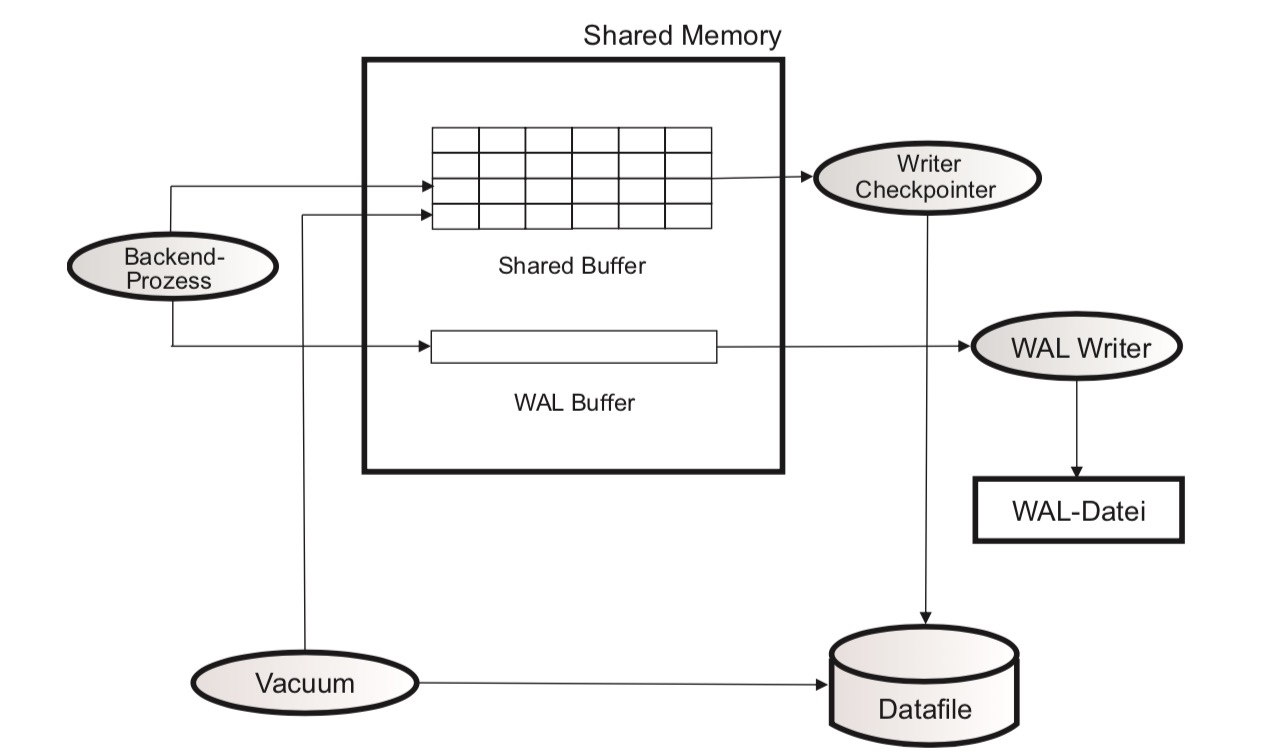
\includegraphics[width = \linewidth]{images/postgresArchitektur.jpg}
    \caption{Postgres Architektur}
    \label{Postgres Architektur}

\end{figure}
\section{Graph-Datenbanken im praktischen Einsatz: OLTP}
\lstsetsql
\begin{lstlisting}[language=SQL,caption=CSV Input,frame=single, label={copy}]
    \copy Beitraege
    FROM './data/Beitraege.csv' DELIMITER ',' CSV HEADER;
\end{lstlisting}

\begin{lstlisting}[language=SQL,caption=Anlegen der Tabelle facebook-profiles,frame=single, label={facebookProfiles}]
    create TABLE IF NOT EXISTS profiles_facebook(
        ID INTEGER PRIMARY KEY,
        first VARCHAR(50),
        last VARCHAR(50),
        gender GENDER,
        birth DATE,
        country VARCHAR(50)
    );
\end{lstlisting}

\begin{lstlisting}[language=SQL,caption=Anlegen der Tabelle facebook-relation,frame=single, label={relationFacebook}]
    CREATE TABLE IF NOT EXISTS relation_facebook(
        src INTEGER REFERENCES profiles_facebook(ID),
        dst INTEGER REFERENCES profiles_facebook(ID),
        type VARCHAR(50),
        date DATE
    );
\end{lstlisting}

\begin{lstlisting}[language=SQL,caption=Hinzufügen von Fremdschlüsseln,frame=single, label={foreignKey}]
    \copy profiles_facebook_tmp(first,last,gender,birth,country) FROM '/data/WS2018/facebook-profiles' DELIMITER ',' CSV HEADER;
    INSERT INTO profiles_facebook (ID, first, last, gender, birth, country)
    SELECT ID-1, first, last, gender, birth, country from profiles_facebook_tmp;
\end{lstlisting}

\begin{lstlisting}[language=SQL,caption=Erstellen von partitionierten Tabellen mit Index facebook,frame=single, label={parttableindexfacebook}]
    CREATE TABLE IF NOT EXISTS relation_facebook_partitioned(
        src INTEGER REFERENCES profiles_facebook(ID),
        dst INTEGER REFERENCES profiles_facebook(ID),
        type VARCHAR(50),
        date DATE
    )PARTITION BY RANGE(src);

    CREATE INDEX fb_part_src ON relation_facebook_partitioned (src);
    CREATE INDEX fb_part_dst ON relation_facebook_partitioned (dst);

    CREATE TABLE relation_facebook_partitioned_0 PARTITION OF relation_facebook_partitioned
    FOR VALUES FROM (0) TO (23000);
    CREATE TABLE relation_facebook_partitioned_1 PARTITION OF relation_facebook_partitioned
    FOR VALUES FROM (23000) TO (46000);
    CREATE TABLE relation_facebook_partitioned_2 PARTITION OF relation_facebook_partitioned
    FOR VALUES FROM (46000) TO (69000);
    CREATE TABLE relation_facebook_partitioned_3 PARTITION OF relation_facebook_partitioned
    FOR VALUES FROM (69000) TO (92000);
\end{lstlisting}

\begin{lstlisting}[language=SQL,caption=Erstellen von Indexen auf relation Tabelle facebook,frame=single, label={indexfacebook}]
    CREATE INDEX fb_dst ON relation_facebook_with_index (dst);
    CREATE INDEX fb_src ON relation_facebook_with_index (src);
\end{lstlisting}

\begin{lstlisting}[language=SQL,caption=Erstellen von partitionierten Tabellen mit Index youtube,frame=single, label={parttableindexyoutube}]
    CREATE TABLE IF NOT EXISTS relation_youtube_partitioned(
        src INTEGER REFERENCES profiles_youtube(ID),
        dst INTEGER REFERENCES profiles_youtube(ID),
        type VARCHAR(50),
        date DATE
    )PARTITION BY RANGE(src);

    CREATE INDEX yt_part_src ON relation_youtube_partitioned (src);
    CREATE INDEX yt_part_dst ON relation_youtube_partitioned (dst);

    CREATE TABLE relation_youtube_partitioned_0 PARTITION OF relation_youtube_partitioned
    FOR VALUES FROM (0) TO (800000);
    CREATE TABLE relation_youtube_partitioned_1 PARTITION OF relation_youtube_partitioned
    FOR VALUES FROM (800001) TO (1600000);
    CREATE TABLE relation_youtube_partitioned_2 PARTITION OF relation_youtube_partitioned
    FOR VALUES FROM (1600001) TO (2400000);
    CREATE TABLE relation_youtube_partitioned_3 PARTITION OF relation_youtube_partitioned
    FOR VALUES FROM (2400001) TO (3200000);
\end{lstlisting}

\begin{lstlisting}[language=SQL,caption=Erstellen von Indexen auf relation Tabelle youtube,frame=single, label={indexyoutube}]
    CREATE INDEX yt_dst ON relation_youtube_with_index (dst);
    CREATE INDEX yt_src ON relation_youtube_with_index (src);
\end{lstlisting}

\begin{lstlisting}[language=SQL,caption=Erstellen von partitionierten Tabellen mit Index livejournal,frame=single, label={parttableindexlivejournal}]
    CREATE TABLE IF NOT EXISTS relation_livejournal_partitioned(
        src INTEGER REFERENCES profiles_livejournal(ID),
        dst INTEGER REFERENCES profiles_livejournal(ID),
        type VARCHAR(50),
        date DATE
    )PARTITION BY RANGE(src);

    CREATE INDEX lj_part_src ON relation_livejournal_partitioned (src);
    CREATE INDEX lj_part_dst ON relation_livejournal_partitioned (dst);

    CREATE TABLE relation_livejournal_partitioned_0 PARTITION OF relation_livejournal_partitioned
    FOR VALUES FROM (0) TO (10000000);
    CREATE TABLE relation_livejournal_partitioned_1 PARTITION OF relation_livejournal_partitioned
    FOR VALUES FROM (10000000) TO (20000000);
    CREATE TABLE relation_livejournal_partitioned_2 PARTITION OF relation_livejournal_partitioned
    FOR VALUES FROM (20000000) TO (30000000);
    CREATE TABLE relation_livejournal_partitioned_3 PARTITION OF relation_livejournal_partitioned
    FOR VALUES FROM (30000000) TO (40000000);
\end{lstlisting}

\begin{lstlisting}[language=SQL,caption=Erstellen von Indexen auf relation Tabelle livejournal,frame=single, label={indexlivejournal}]
    CREATE INDEX lj_src ON relation_livejournal_with_index (src);
    CREATE INDEX lj_dst ON relation_livejournal_with_index (dst);
\end{lstlisting}

\begin{lstlisting}[language=SQL,caption=Erstellen von partitionierten Tabellen mit Index epinion,frame=single, label={parttableindexepinion}]
    CREATE TABLE IF NOT EXISTS relation_epinions_partitioned(
        src INTEGER REFERENCES profiles_epinions(ID),
        dst INTEGER REFERENCES profiles_epinions(ID),
        type VARCHAR(50),
        date DATE
    )PARTITION BY RANGE(src);

    CREATE INDEX ep_part_src ON relation_epinions_partitioned (src);
    CREATE INDEX ep_part_dst ON relation_epinions_partitioned (dst);

    CREATE TABLE relation_epinions_partitioned_0 PARTITION OF relation_epinions_partitioned
    FOR VALUES FROM (0) TO (102000);
    CREATE TABLE relation_epinions_partitioned_1 PARTITION OF relation_epinions_partitioned
    FOR VALUES FROM (102000) TO (204000);
    CREATE TABLE relation_epinions_partitioned_2 PARTITION OF relation_epinions_partitioned
    FOR VALUES FROM (204000) TO (306000);
    CREATE TABLE relation_epinions_partitioned_3 PARTITION OF relation_epinions_partitioned
    FOR VALUES FROM (306000) TO (408000);
\end{lstlisting}

\begin{lstlisting}[language=SQL,caption=Erstellen von Indexen auf relation Tabelle epinion,frame=single, label={indexepinion}]
    CREATE INDEX ep_dst ON relation_epinions_with_index (dst);
    CREATE INDEX ep_src ON relation_epinions_with_index (src);
\end{lstlisting}

\begin{lstlisting}[language=SQL,caption=Erstellen von partitionierten Tabellen mit wikivote epinion,frame=single, label={parttableindexwikivote}]
    CREATE TABLE IF NOT EXISTS relation_wiki_vote_partitioned(
        src INTEGER REFERENCES profiles_wiki_vote(ID),
        dst INTEGER REFERENCES profiles_wiki_vote(ID),
        type VARCHAR(50),
        date DATE
    )PARTITION BY RANGE(src);

    CREATE INDEX wv_part_src ON relation_wiki_vote_partitioned (src);
    CREATE INDEX wv_part_dst ON relation_wiki_vote_partitioned (dst);

    CREATE TABLE relation_wiki_vote_partitioned_0 PARTITION OF relation_wiki_vote_partitioned
    FOR VALUES FROM (0) TO (30000);
    CREATE TABLE relation_wiki_vote_partitioned_1 PARTITION OF relation_wiki_vote_partitioned
    FOR VALUES FROM (30000) TO (60000);
    CREATE TABLE relation_wiki_vote_partitioned_2 PARTITION OF relation_wiki_vote_partitioned
    FOR VALUES FROM (60000) TO (90000);
    CREATE TABLE relation_wiki_vote_partitioned_3 PARTITION OF relation_wiki_vote_partitioned
    FOR VALUES FROM (90000) TO (120000);
\end{lstlisting}

\begin{lstlisting}[language=SQL,caption=Erstellen von Indexen auf relation Tabelle wikivote,frame=single, label={indexwikivote}]
    CREATE INDEX wv_src ON relation_wiki_vote_with_index (src);
    CREATE INDEX wv_dst ON relation_wiki_vote_with_index (dst);
\end{lstlisting}

\begin{lstlisting}[language=SQL,caption=Erstellen der Indexe für die relation Tabelle facebook,frame=single, label={indexfacebook}]
    CREATE INDEX fb_dst ON relation_facebook_with_index (dst);
    CREATE INDEX fb_src ON relation_facebook_with_index (src);
\end{lstlisting}

\begin{lstlisting}[language=SQL,caption = Verschachteltes SELECT Statement,frame=single,label={SELECT} ]
    SELECT DISTINCT(dst) FROM team22.relation_facebook WHERE src IN(
        SELECT DISTINCT(dst) FROM team22.relation_facebook WHERE src IN(
            SELECT DISTINCT(dst)FROM team22.relation_facebook WHERE src IN(1)
        )
    )
\end{lstlisting}

\begin{lstlisting}[language=SQL,caption = Rekursiver JOIN,frame=single, label={JOIN} ]
    SELECT DISTINCT(rf3.dst)
    FROM public.relation_facebook rf1,
    public.relation_facebook rf2,
    public.relation_facebook rf3
    WHERE rf2.src = rf1.dst
    AND rf3.src = rf2.dst
    AND rf1.src = 765;
\end{lstlisting}
\newpage
\begin{lstlisting}[language=SQL,caption = Selbstgeschriebenes Stored Procedure,frame=single, label={recursiveFunction} ]
    CREATE OR REPLACE FUNCTION recursivesearch(tInput integer[], iRecursionDepth integer, sTable text) RETURNS SETOF integer AS $$
    Declare
    intermDst_ integer[];
    iCount integer;
    BEGIN
    --iRecursionDepth = iRecursionDepth + 1;
    CREATE TEMPORARY TABLE intermDst AS SELECT * FROM unnest(tInput);
    EXECUTE 'CREATE TEMPORARY TABLE intermDst1 AS SELECT DISTINCT(dst) FROM ' || sTable || ' WHERE src IN (SELECT * FROM intermDst)';
    -- Does not return from function!
    return query SELECT * FROM intermDst1;
    -- Does not return from function!
    intermDst_ := ARRAY(SELECT * FROM intermDst1);
    raise notice 'timestamp: %', clock_timestamp();
    SELECT count(*) INTO iCount FROM intermDst;
    raise notice 'Count Table: %', iCount;
    DROP TABLE intermDst;
    DROP TABLE intermDst1;
    -- As recursion depth is 5
    if iRecursionDepth > 1 THEN
    return query SELECT * FROM recursivesearch(intermDst_, iRecursionDepth - 1, sTable);
    ELSE
    RETURN;
    END IF;
    END;
    $$ LANGUAGE plpgsql;
\end{lstlisting}

\begin{lstlisting}[language=SQL,caption = SQL Standard Generisch,frame=single, label={StandardSQLGenerisch} ]
    CREATE OR REPLACE FUNCTION selectWithUnionSourceCodeGenerator_withDepth(sTable text, startingNode integer, depth integer ) RETURNS SETOF integer AS $$
    Declare
    intermDst_ integer[];
    tStatement text;
    tSelectStatement text;
    tWithStatement text;
    tUnionStatement text;
    tWithStatementClose text;
    BEGIN
    tWithStatement := 'WITH RECURSIVE graphtraverse(src, dst, lvl) AS(';
    tSelectStatement := 'SELECT src ,dst, 1 as lvl FROM ' || sTable || ' WHERE src ='||startingNode;
    tUnionStatement := ' UNION SELECT p1.src,p1.dst,p.lvl+1 as lvl FROM graphtraverse p, ' || sTable || ' p1 WHERE p1.src IN ( p.dst ) and lvl<'||depth;
    tWithStatementClose := ') SELECT DISTINCT(dst) FROM graphtraverse';
    tStatement := tWithStatement || tSelectStatement || tUnionStatement || tWithStatementClose;
    raise notice 'Execute String %', tStatement;
    return query EXECUTE tStatement;
    END;
    $$ LANGUAGE plpgsql;
\end{lstlisting}

\begin{lstlisting}[language=SQL,caption = SQL Standard,frame=single, label={StandardSQL} ]
    WITH RECURSIVE graphtraverse(src, dst, lvl) AS(
    SELECT src ,dst, 1 as lvl FROM public.relation_facebook WHERE src =765
    UNION
    SELECT p1.src,p1.dst,p.lvl+1 as lvl FROM graphtraverse p, relation_facebook p1 WHERE p1.src IN ( p.dst ) and lvl<5
    ) SELECT DISTINCT(dst) FROM graphtraverse order by dst;
\end{lstlisting}

\begin{lstlisting}[language=SQL,caption = Ausführungsplan Standard SQL,frame=single, label={AusführungsplanCTEFacebook} ]
    Sort  (cost=15300.01..15300.51 rows=200 width=4) (actual time=17.613..17.622 rows=321 loops=1)
    Sort Key: graphtraverse.dst
    Sort Method: quicksort  Memory: 40kB
    CTE graphtraverse
    ->  Recursive Union  (cost=0.29..14814.87 rows=21133 width=12) (actual time=0.016..15.903 rows=6056 loops=1)
        ->  Index Scan using indexsrc on relation_facebook  (cost=0.29..44.00 rows=23 width=12) (actual time=0.015..0.020 rows=27 loops=1)
        Index Cond: (src = 765)
        ->  Nested Loop  (cost=0.29..1434.82 rows=2111 width=12) (actual time=0.019..2.130 rows=8173 loops=5)
            ->  WorkTable Scan on graphtraverse p  (cost=0.00..5.17 rows=77 width=8) (actual time=0.017..0.069 rows=729 loops=5)
            Filter: (lvl < 5)
            Rows Removed by Filter: 482
        ->  Index Scan using indexsrc on relation_facebook p1  (cost=0.29..18.23 rows=27 width=8) (actual time=0.001..0.002 rows=11 loops=3645)
            Index Cond: (src = p.dst)
    ->  HashAggregate  (cost=475.49..477.49 rows=200 width=4) (actual time=17.548..17.571 rows=321 loops=1)
        Group Key: graphtraverse.dst
        ->  CTE Scan on graphtraverse  (cost=0.00..422.66 rows=21133 width=4) (actual time=0.017..16.771 rows=6056 loops=1)
    Planning Time: 0.105 ms
    Execution Time: 17.813 ms
\end{lstlisting}

\begin{lstlisting}[language=SQL,caption = Ausführungsplan verschachteltes SELECT,frame=single, label={AusführungsplanCascadeSELECT} ]
    HashAggregate  (cost=6623.97..6659.95 rows=3598 width=4) (actual time=27.019..27.049 rows=317 loops=1)
    Group Key: relation_facebook.dst
    ->  Hash Join  (cost=4727.16..6403.39 rows=88234 width=4) (actual time=20.593..26.743 rows=2411 loops=1)
    Hash Cond: (relation_facebook.src = relation_facebook_1.dst)
        ->  Seq Scan on relation_facebook  (cost=0.00..1444.34 rows=88234 width=8) (actual time=0.008..3.889 rows=88234 loops=1)
        ->  Hash  (cost=4682.18..4682.18 rows=3598 width=4) (actual time=18.021..18.021 rows=195 loops=1)
            Buckets: 4096  Batches: 1  Memory Usage: 39kB
            ->  HashAggregate  (cost=4610.22..4646.20 rows=3598 width=4) (actual time=17.976..18.000 rows=195 loops=1)
                Group Key: relation_facebook_1.dst
                ->  Hash Join  (cost=2713.40..4389.64 rows=88234 width=4) (actual time=11.821..17.797 rows=1709 loops=1)
                    Hash Cond: (relation_facebook_1.src = relation_facebook_2.dst)
                        ->  Seq Scan on relation_facebook relation_facebook_1  (cost=0.00..1444.34 rows=88234 width=8) (actual time=0.002..3.916 rows=88234 loops=1)
                        ->  Hash  (cost=2668.43..2668.43 rows=3598 width=4) (actual time=9.177..9.177 rows=144 loops=1)
                            Buckets: 4096  Batches: 1  Memory Usage: 38kB
                            ->  HashAggregate  (cost=2596.47..2632.45 rows=3598 width=4) (actual time=9.140..9.161 rows=144 loops=1)
                                Group Key: relation_facebook_2.dst
                                ->  Hash Join  (cost=876.96..2553.22 rows=17301 width=4) (actual time=2.942..9.020 rows=1280 loops=1)
                                    Hash Cond: (relation_facebook_2.src = relation_facebook_3.dst)
                                    ->  Seq Scan on relation_facebook relation_facebook_2  (cost=0.00..1444.34 rows=88234 width=8) (actual time=0.002..4.163 rows=88234 loops=1)
                                    ->  Hash  (cost=869.07..869.07 rows=631 width=4) (actual time=0.276..0.276 rows=88 loops=1)
                                        Buckets: 1024  Batches: 1  Memory Usage: 12kB
                                        ->  HashAggregate  (cost=856.45..862.76 rows=631 width=4) (actual time=0.259..0.268 rows=88 loops=1)
                                            Group Key: relation_facebook_3.dst
                                                ->  Nested Loop  (cost=44.35..854.88 rows=631 width=4) (actual time=0.022..0.199 rows=629 loops=1)
                                                    ->  HashAggregate  (cost=44.05..44.28 rows=23 width=4) (actual time=0.018..0.021 rows=27 loops=1)
                                                    Group Key: relation_facebook_4.dst
                                                    ->  Index Scan using indexsrc on relation_facebook relation_facebook_4  (cost=0.29..44.00 rows=23 width=4) (actual time=0.009..0.012 rows=27 loops=1)
                                                        Index Cond: (src = 765)
                                        ->  Index Scan using indexsrc on relation_facebook relation_facebook_3  (cost=0.29..34.96 rows=27 width=8) (actual time=0.002..0.005 rows=23 loops=27)
                                            Index Cond: (src = relation_facebook_4.dst)
    Planning Time: 0.170 ms
    Execution Time: 27.113 ms


\end{lstlisting}

\begin{lstlisting}[language=SQL,caption = Ausführungsplan INNER JOIN,frame=single, label={AusführungsplanINNERJOIN} ]
    HashAggregate  (cost=172324.88..172360.86 rows=3598 width=4) (actual time=156.786..156.823 rows=317 loops=1)
    Group Key: rf5.dst
    Buffers: shared hit=2654
    ->  Merge Join  (cost=38989.73..153806.87 rows=7407207 width=4) (actual time=33.728..105.213 rows=572149 loops=1)
    Merge Cond: (rf5.src = rf4.dst)
    Buffers: shared hit=2654
    ->  Index Scan using indexsrc on relation_facebook rf5  (cost=0.29..3539.96 rows=88234 width=8) (actual time=0.004..3.466 rows=33654 loops=1)
    Buffers: shared hit=331
    ->  Sort  (cost=38972.52..39749.91 rows=310956 width=4) (actual time=30.171..50.861 rows=579169 loops=1)
    Sort Key: rf4.dst
    Sort Method: quicksort  Memory: 6709kB
    Buffers: shared hit=2323
    ->  Merge Join  (cost=2353.66..10603.46 rows=310956 width=4) (actual time=9.093..21.946 rows=77587 loops=1)
    Merge Cond: (rf3.dst = rf4.src)
    Buffers: shared hit=2323
    ->  Sort  (cost=2333.95..2366.58 rows=13054 width=4) (actual time=3.176..3.593 rows=8177 loops=1)
    Sort Key: rf3.dst
    Sort Method: quicksort  Memory: 576kB
    Buffers: shared hit=1993
    ->  Nested Loop  (cost=0.88..1441.56 rows=13054 width=4) (actual time=0.012..2.289 rows=8177 loops=1)
    Buffers: shared hit=1993
    ->  Nested Loop  (cost=0.58..854.36 rows=548 width=4) (actual time=0.009..0.156 rows=629 loops=1)
    Buffers: shared hit=89
    ->  Index Scan using indexsrc on relation_facebook rf1  (cost=0.29..44.00 rows=23 width=4) (actual time=0.004..0.008 rows=27 loops=1)
    Index Cond: (src = 765)
    Buffers: shared hit=3
    ->  Index Scan using indexsrc on relation_facebook rf2  (cost=0.29..34.96 rows=27 width=8) (actual time=0.001..0.003 rows=23 loops=27)
    Index Cond: (src = rf1.dst)
    Buffers: shared hit=86
    ->  Index Scan using indexsrc on relation_facebook rf3  (cost=0.29..0.80 rows=27 width=8) (actual time=0.001..0.002 rows=13 loops=629)
    Index Cond: (src = rf2.dst)
    Buffers: shared hit=1904
    ->  Materialize  (cost=0.29..3760.54 rows=88234 width=8) (actual time=0.004..8.301 rows=109531 loops=1)
    Buffers: shared hit=330
    ->  Index Scan using indexsrc on relation_facebook rf4  (cost=0.29..3539.96 rows=88234 width=8) (actual time=0.003..3.863 rows=33653 loops=1)
    Buffers: shared hit=330
    Planning Time: 0.627 ms
    Execution Time: 157.021 ms

\end{lstlisting}

\section{Graph-Datenbanken im praktischen Einsatz: OLAP}
%\chapter{Anhang}
%Appendix
%
%% #####
%% # list of table, list of figures, and list of listings in ToC
%% #####
%\newpage
%\addcontentsline{toc}{chapter}{Abbildungsverzeichnis}
%\listoffigures
%\newpage
%\addcontentsline{toc}{chapter}{Tabellenverzeichnis}
%\listoftables
%\newpage
%\addcontentsline{toc}{chapter}{Listings}
%\lstlistoflistings
%
%% #####
%% # List of Abbreviations
%% #####
%\phantomsection
%\addcontentsline{toc}{chapter}{Abkürzungsverzeichnis}
%\renewcommand\refname{Abkürzungsverzeichnis}
%\chapter*{Abkürzungsverzeichnis}
%\begin{acronym}[RDBMS] % längste Abkürzung steht in eckigen Klammern
    \setlength{\itemsep}{-\parsep} % geringerer Zeilenabstand
    \acro{ACID}{Atomicity, Consistency, Isolation, Durability}
    \acro{API}{Application Programming Interface}
    \acro{APT}{Advanced Package Tool}
%    \acro{BASE}{Basically Available, Soft State, Eventual Consistency}
%    \acro{BG}{Barahmand Ghandeharizadeh}
%    \acro{CAP}{Consistency Availibiltiy Partition Tolerance}
%    \acro{CLI}{Command-Line Interface}
%    \acro{CPU}{Central Processing Unit}
    \acro{CRUD}{Create, Read, Update, Delete}
%    \acro{DBA}{Datenbankadministrator}
%    \acro{DBS}{Datenbanksystem}
%    \acrodefplural{DBS}[DBS]{Datenbanksysteme}
%    \acrodefplural{HDD}[HDDs]{Hard Disk Drive}
%    \acrodefplural{SSD}[SSDs]{Solid State Drive}
%    \acro{DNS}{Domain Name System}
%    \acro{DTD}{Document Type Definition}
%    \acro{GUI}{Graphical User Interface}
%    \acro{HDD}{Hard Disk Drive}
%    \acro{HTTP}{HyperText Transfer Protocol}
    \acro{IP}{Internet Protocol}
    \acro{TCP}{Transmission Control Protocol}
%    \acro{JDBC}{Java Database Connectivity}
%    \acro{JSON}{JavaScript Object Notation}
    \acro{MVCC}{Multiversion Concurrency Control Modell}
    \acro{NoSQL}{Not only SQL}
    \acro{OLTP}{Online Transaction Processing}
    \acro{RPM}{Red Hat Package Manager}
%    \acro{RDBMS}{Relational Database Management System}
%    \acro{RFC}{Request For Comments}
%    \acro{SLA}{Service Level Agreement}
%    \acro{SPEC}{Standard Performance Evaluation Corporation}
    \acro{SQL}{Structured Query Language}
%    \acro{SSD}{Solid State Drive}
%    \acro{TPC}{Transaction Processing Performance Council}
%    \acro{UML}{Unified Markup Language}
%    \acro{XML}{Extensible Markup Language}
%    \acro{YCSB}{Yahoo! Cloud Serving Benchmark}
\end{acronym}

%\newpage

% #####
% # load the bibliography
% #####
\bibliography{bibliography}

% #####
% # load the sworn declaration
% #####
\chapter*{Eidesstattliche Erklärung}\markboth{Eidesstattliche Erklärung}{}
  \addcontentsline{toc}{chapter}{Eidesstattliche Erklärung}
Ich versichere an Eides Statt durch meine eigenhändige Unterschrift, dass
ich die vorliegende Arbeit selbstständig und ohne fremde Hilfe angefertigt
habe. Alle Stellen, die wörtlich oder dem Sinn nach auf Publikationen oder
Vorträgen anderer Autoren beruhen, sind als solche kenntlich gemacht.
Ich versichere außerdem, dass ich keine andere als die angegebene
Literatur verwendet habe. Diese Versicherung bezieht sich auch auf alle in
der Arbeit enthaltenen Zeichnungen, Skizzen, bildlichen Darstellungen und
dergleichen.
\\
\\
Die Arbeit wurde bisher keiner anderen Prüfungsbehörde vorgelegt und
auch noch nicht veröffentlicht.
\vspace{3cm}

\centering
\begin{tabular}{p{10mm}>{\centering\arraybackslash}p{50mm}p{10mm}
>{\centering\arraybackslash}p{50mm}p{10mm}}
&\textit{\large \TOWN,}&&& \\
&\textit{\large den \today}&&\hrulefill& \\
&\small Ort, Datum&&\small \AUTHOR&
\end{tabular}
% end of the document
\end{document}
